\documentclass[11pt,a4paper,twocolumn]{article}
\usepackage[utf8]{inputenc}
\usepackage{amsmath}
\usepackage{graphicx}
\usepackage{hyperref}
\usepackage{setspace}
\usepackage{enumerate}
\usepackage[inline]{enumitem}   
\title{Assignment9}
\author{Aravind A Anil}
\date{\today}
\begin{document}
\maketitle
\begin{flushleft}
\textbf{Q.The probability that a K-digit number does not contain the digits 0,5 or 9 is?:}
\end{flushleft}
\begin{enumerate*}[label=\alph*)]
    \item $.3^{k}$\hspace{.5cm}
    \item $.6^{k}$\hspace{.5cm}
    \item $.7^{k}$\hspace{.5cm}
    \item $.9^{k}$\hspace{.5cm}
\end{enumerate*}\\[5pt]
\textbf{Solution:}Let $Z_{i}$ $\in$ (0,1,2,3,4,5,6,7,8,9) represents the $i^{th}$ position of k digit number\\
\begin{equation*}
 Pr(Z_{i}\notin{0,5,9})=\frac{7}{10}   
\end{equation*}
If a K-digit number does not contain 0,5,9 it can be written as\\
$Pr(Z_{1}$ $\notin$ ${0,5,9}$,$Z_{2}$ $\notin$ ${0,5,9}$,$Z_{3}$ $\notin$ ${0,5,9}$,......$Z_{k}$ $\notin$ ${0,5,9}$)\\
Since getting digit in different places of a number is a independent event it can be written as
\begin{align*}
\hspace{-3cm}
&=Pr(Z_{1} \notin {0,5,9},Z_{2} \notin {0,5,9},Z_{3} \notin {0,5,9}....\\
&\quad......Z_{k} \notin {0,5,9})\\
&=Pr(Z_{1} \notin {0,5,9})\times Pr(Z_{2} \notin {0,5,9})\times Pr(Z_{3} \notin {0,5,9}) \\
&\quad\times......Pr(Z_{k} \notin {0,5,9})\\
&=\prod_{i=1}^{k}.7\\
&=.7^{k}
\end{align*}
So,\textbf{Answer is option C}
\begin{figure}
    \centering
    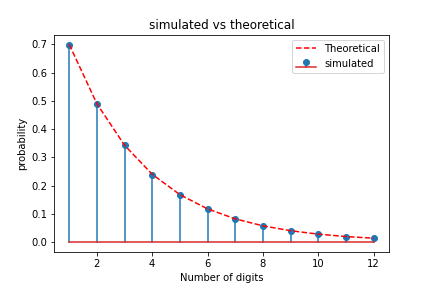
\includegraphics[width=10cm]{theoretical vs simulated.png}
    \caption{theoretical vs simulated}
    \label{fig:my_label}
\end{figure}
\end{document}
